\section{Area Studi Sacramento Valley}
Area studi penelitian ini adalah Sacramento Valley dalam daerah Central Valley, California, pada koordinat geografis ($122^{\circ}4'41''$ BB hingga $121^{\circ}34'31''$ BB, $38^{\circ}45'14''$ LU hingga $39^{\circ}10'29''$ LU) dengan total luas area 2.038,08 km$^2$. 
Kawasan ini memiliki bentang alam dan jenis tanaman yang sangat beragam karena variasi iklim dan topografinya, juga menjadi salah satu wilayah pertanian paling produktif di Amerika Serikat dengan jenis tanaman pertanian yang beragam. 
Iklim di wilayah ini termasuk minim hujan di musim panas, sehingga memungkinkan pengamatan spektral tanaman sepanjang musim tanam \citep{yuan2021}. 

\section{Pengumpulan Data}
Data pada penelitian ini menggunakan citra satelit Sentinel-2 dan data label tutupan lahan dari Cropland Data Layer (CDL). 
Data citra diambil dari koleksi Sentinel-2 Surface Reflectance (COPERNICUS/S2\_SR\_HARMONIZED) melalui platform Google Earth Engine (GEE) dengan batas persentase awan kurang dari 10\% pada area studi. 
Citra dikumpulkan secara multi-temporal sepanjang tahun 2022, 2023, dan 2024 dengan interval pengambilan setiap 15 hari sekali. 
Periode akuisisi mencakup satu tahun penuh, menghasilkan total 72 citra komposit yang terdiri dari 24 citra pada 2022, 23 citra pada 2023, dan 25 citra pada 2024. 
Terdapat tiga interval citra yang melebihi batas persentase awan, sehingga tidak digunakan sebagai dataset. 

Untuk mendapatkan citra multispektral, dipilih sembilan band (B2, B3, B4, B5, B6, B7, B8, B11, B12) yang relevan terhadap karakteristik vegetasi. 
Sementara itu, data label diperoleh dari dataset CDL tahun 2022, 2023, dan 2024 yang diunduh melalui situs resmi USDA NASS yang terdiri dari 134 kelas dengan resolusi spasial 30 meter per piksel.

\section{Eksplorasi Data}
\subsection{Visualisasi Citra}
Visualisasi citra Sentinel-2 mencakup citra True Color (RGB) yang merupakan representasi visual yang tampak pada mata manusia berdasarkan Band B4 (Red), Band B3 (Green), dan Band B2 (Blue). 
Selain itu, ditampilkan juga band multispektral yang digunakan untuk menyoroti perbedaan pantulan (\textit{reflectance}) pada panjang gelombang tertentu.

\subsection{Statistik Deskriptif}
Setiap citra mencakup sekitar 11.810.282 piksel. 
Pada data preprocessing, akan dilakukan pembagian patch berukuran $256\times256$ piksel, sehingga setiap citra akan menghasilkan sekitar 180 patch. 
Total citra yang diambil dari tahun 2022--2024 adalah 72 citra, sehingga akan diperoleh total 12.960 patch.

\subsection{Data Label CDL}
Dataset CDL tahun 2022 pada area studi memiliki 72 kelas aktif yang terbagi menjadi 48 kelas tanaman (\textit{cropland}) dan 16 kelas non-tanaman (permukiman, perairan, lahan basah, semak, dan lainnya).
Lahan pertanian (\textit{cropland}) mencakup 83,8\% dari total area studi, sedangkan sisanya (16,2\%) merupakan lahan non-pertanian.
Label CDL menggunakan proyeksi EPSG:5070 (NAD83/Conus Albers) dengan resolusi spasial 30 meter per piksel, sedangkan Sentinel-2 menggunakan proyeksi EPSG:4326 (WGS84) dengan resolusi spasial $\approx$10 meter per piksel, sehingga diperlukan proses reprojektion dan \textit{resampling} sebelum digunakan sebagai label pelatihan.

\subsubsection{Distribusi Kelas CDL di Area Studi}

Distribusi kelas CDL pada area studi dianalisis berdasarkan jumlah piksel hasil reprojektion ke grid Sentinel-2 ($5.596 \times 4.684$ piksel, ukuran piksel $7{,}78 \times 10{,}00$ m$^2 \approx 77{,}8$ m$^2$/piksel).
Tabel~\ref{tab:cdl_top30} menyajikan 30 kelas dengan cakupan tertinggi beserta konversinya ke satuan hektar dan kilometer persegi.

\begin{table}[htbp]
\centering
\caption{30 Kelas CDL Teratas Berdasarkan Cakupan Area di Area Studi (2022)}
\label{tab:cdl_top30}
\resizebox{\textwidth}{!}{%
\begin{tabular}{rlrrrr}
\hline
\textbf{No.} & \textbf{Nama Kelas} & \textbf{ID} & \textbf{Piksel} & \textbf{Area (ha)} & \textbf{Area (km$^2$)} \\
\hline
1  & Fallow/Idle Cropland       & 61  & 7.426.247 & 57.742,5 & 577,42 \\
2  & Almonds                    & 75  & 3.011.056 & 23.412,3 & 234,12 \\
3  & Walnuts                    & 76  & 2.387.806 & 18.566,3 & 185,66 \\
4  & Tomatoes                   & 54  & 1.942.579 & 15.104,4 & 151,04 \\
5  & Rice                       & 3   & 1.731.503 & 13.463,2 & 134,63 \\
6  & Grass/Pasture              & 176 & 1.359.253 & 10.568,8 & 105,69 \\
7  & Winter Wheat               & 24  & 1.231.983 &  9.579,2 &  95,79 \\
8  & Sunflower                  & 6   &   913.565 &  7.103,4 &  71,03 \\
9  & Developed/Low Intensity    & 122 &   632.042 &  4.914,4 &  49,14 \\
10 & Alfalfa                    & 36  &   575.672 &  4.476,1 &  44,76 \\
11 & Developed/Med Intensity    & 123 &   570.466 &  4.435,6 &  44,36 \\
12 & Plums                      & 220 &   560.637 &  4.359,2 &  43,59 \\
13 & Developed/Open Space       & 121 &   536.853 &  4.174,3 &  41,74 \\
14 & Herbaceous Wetlands        & 195 &   381.008 &  2.962,5 &  29,63 \\
15 & Other Hay/Non Alfalfa      & 37  &   375.842 &  2.922,3 &  29,22 \\
16 & Open Water                 & 111 &   331.675 &  2.578,9 &  25,79 \\
17 & Grapes                     & 69  &   327.883 &  2.549,4 &  25,49 \\
18 & Safflower                  & 33  &   240.323 &  1.868,6 &  18,69 \\
19 & Pistachios                 & 204 &   203.826 &  1.584,8 &  15,85 \\
20 & Woody Wetlands             & 190 &   173.782 &  1.351,2 &  13,51 \\
21 & Developed/High Intensity   & 124 &   127.919 &    994,6 &   9,95 \\
22 & Watermelons                & 48  &   118.805 &    923,8 &   9,24 \\
23 & Oats                       & 28  &    96.406 &    749,6 &   7,50 \\
24 & Shrubland                  & 152 &    95.610 &    743,4 &   7,43 \\
25 & Barley                     & 21  &    88.582 &    688,8 &   6,89 \\
26 & Corn                       & 1   &    86.009 &    668,8 &   6,69 \\
27 & Olives                     & 211 &    77.289 &    601,0 &   6,01 \\
28 & Prunes                     & 210 &    76.737 &    596,7 &   5,97 \\
29 & Dry Beans                  & 42  &    64.263 &    499,7 &   5,00 \\
30 & Other Crops                & 44  &    63.890 &    496,8 &   4,97 \\
\hline
   & \textit{(+42 kelas minor)} &     & \multicolumn{3}{r}{\textit{cakupan gabungan $<$3\%}} \\
   & \textbf{Total}             &     & \textbf{26.211.664} & \textbf{203.807,7} & \textbf{2.038,08} \\
\hline
\end{tabular}%
}
\end{table}

Rekapitulasi berdasarkan tipe penggunaan lahan disajikan pada Tabel~\ref{tab:cdl_landtype}.

\begin{table}[htbp]
\centering
\caption{Rekapitulasi Cakupan Lahan berdasarkan Tipe Penggunaan}
\label{tab:cdl_landtype}
\begin{tabular}{lrrr}
\hline
\textbf{Tipe Lahan} & \textbf{Area (ha)} & \textbf{Area (km$^2$)} & \textbf{\%} \\
\hline
Tanaman aktif (annual \& perennial crops) & $\approx$103.000 & $\approx$1.030 & 50,5\% \\
Lahan bero (\textit{Fallow/Idle})         &       57.742     &        577     & 28,3\% \\
Non-pertanian (permukiman, air, lahan basah, semak) & $\approx$43.000 & $\approx$430 & 21,2\% \\
\hline
\textbf{Total}                            & \textbf{203.808} & \textbf{2.038} & \textbf{100\%} \\
\hline
\end{tabular}
\end{table}

\subsubsection{Seleksi Kelas Optimal untuk Pelatihan Model}
\label{subsec:class_selection}

Dari 72 kelas CDL yang teridentifikasi di area studi, dilakukan seleksi kelas untuk pelatihan model berdasarkan ambang batas cakupan area minimum $\geq 1\%$ dari total area studi. Visualisasi distribusi kelas dan strategi seleksi ditampilkan pada Gambar~\ref{fig:cdl_class_selection}.

\begin{figure}[htbp]
    \centering
    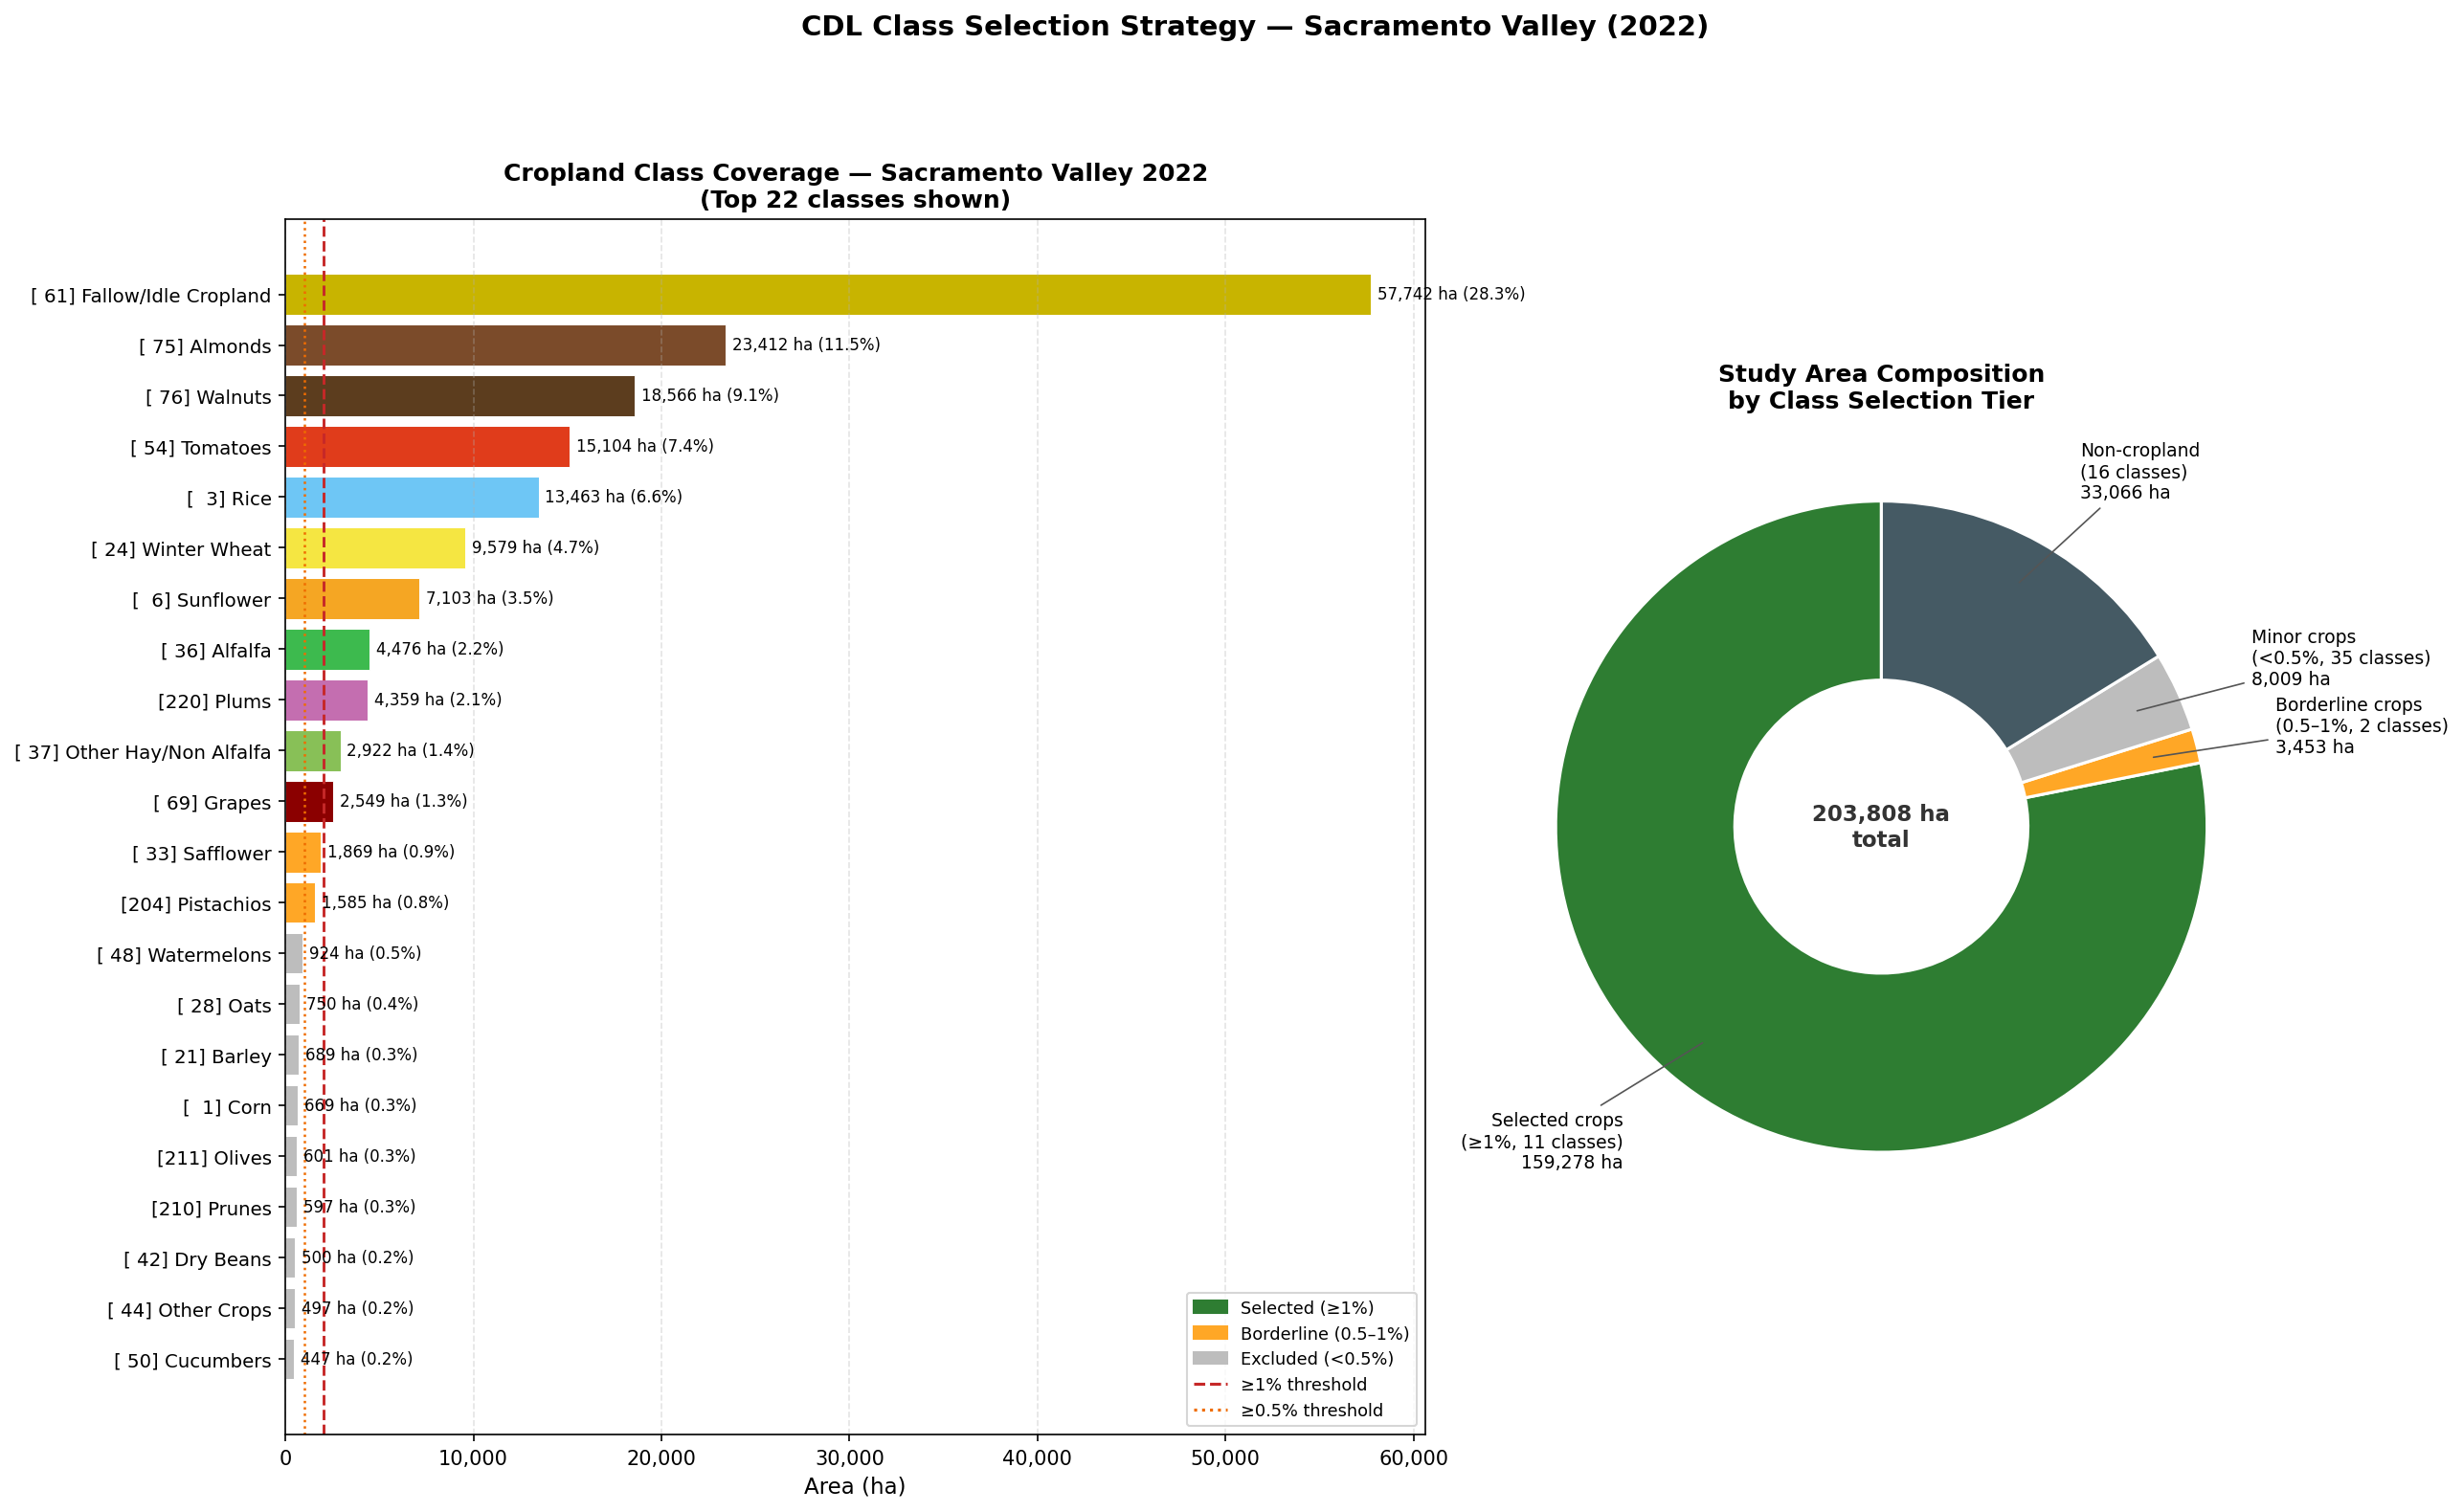
\includegraphics[width=\textwidth]{figures/cdl_class_selection_strategy.png}
    \caption{Distribusi kelas CDL dan strategi seleksi kelas untuk pelatihan model. Kelas dengan cakupan $\geq 1\%$ dipilih sebagai kelas target (hijau), kelas 0{,}5--1\% sebagai kandidat eksperimen lanjutan (oranye), dan kelas $<0{,}5\%$ dikecualikan (abu-abu).}
    \label{fig:cdl_class_selection}
\end{figure}

Tabel~\ref{tab:selected_classes} menampilkan 11 kelas yang terpilih beserta justifikasinya.

\begin{table}[htbp]
\centering
\caption{Kelas CDL Terpilih untuk Pelatihan Model ($\geq 1\%$ cakupan area studi)}
\label{tab:selected_classes}
\begin{tabular}{rlrrrr}
\hline
\textbf{No.} & \textbf{Kelas} & \textbf{ID} & \textbf{\% Tanaman} & \textbf{Area (ha)} & \textbf{Area (km$^2$)} \\
\hline
1  & Fallow/Idle Cropland  & 61  & 33,8\% & 57.742 & 577,42 \\
2  & Almonds               & 75  & 13,7\% & 23.412 & 234,12 \\
3  & Walnuts               & 76  & 10,9\% & 18.566 & 185,66 \\
4  & Tomatoes              & 54  &  8,8\% & 15.104 & 151,04 \\
5  & Rice                  & 3   &  7,9\% & 13.463 & 134,63 \\
6  & Winter Wheat          & 24  &  5,6\% &  9.579 &  95,79 \\
7  & Sunflower             & 6   &  4,2\% &  7.103 &  71,03 \\
8  & Alfalfa               & 36  &  2,6\% &  4.476 &  44,76 \\
9  & Plums                 & 220 &  2,6\% &  4.359 &  43,59 \\
10 & Other Hay/Non Alfalfa & 37  &  1,7\% &  2.922 &  29,22 \\
11 & Grapes                & 69  &  1,5\% &  2.549 &  25,49 \\
-- & Background (lainnya)  & 0   &    --   &    --  &     -- \\
\hline
\multicolumn{3}{l}{\textbf{Total kelas terpilih}} & \textbf{93,3\%} & \textbf{159.278} & \textbf{1.592,8} \\
\hline
\end{tabular}
\end{table}

Terdapat tiga justifikasi ilmiah untuk ambang batas $\geq 1\%$ yang digunakan:

\begin{enumerate}
    \item \textbf{Kecukupan sampel untuk \textit{deep learning}.}
    Kelas dengan cakupan $\geq 1\%$ menempati $\geq 2.038$ ha di area studi.
    Pada ukuran patch $256 \times 256$ piksel dengan resolusi 10 m ($\approx 510$ ha/patch), cakupan tersebut menghasilkan representasi spasial yang memadai dari ratusan petak lahan pertanian yang berbeda, sehingga model dapat mempelajari fitur spektral dan spasial yang dapat digeneralisasi.
    Kelas di bawah 1\% ($<$2.000 ha) umumnya tampil sebagai fragmen poligon yang tersebar dan kecil, sehingga tidak menyediakan keragaman spasial yang cukup untuk pelatihan segmentasi berbasis CNN \citep{alamimachichi2023}.

    \item \textbf{Ketidakseimbangan kelas yang dapat ditangani.}
    Himpunan kelas terpilih menghasilkan rasio ketidakseimbangan maksimum sebesar 22{,}6:1 (Fallow 57.742 ha vs.\ Grapes 2.549 ha).
    Rasio ini masih dapat ditangani dengan teknik standar seperti \textit{inverse-frequency class weighting} atau \textit{Focal Loss} tanpa menyebabkan ketidakstabilan pelatihan.
    Memasukkan kelas di bawah 0{,}5\% akan mendorong rasio ini di atas 100:1, yang melampaui kemampuan koreksi teknik pembobotan standar \citep{luo2024}.

    \item \textbf{Relevansi pertanian Sacramento Valley.}
    Kesebelas kelas yang terpilih merepresentasikan komoditas pertanian dominan Sacramento Valley berdasarkan statistik produksi tahunan USDA NASS \citep{copenhaver2021}:
    \textit{Almonds} dan \textit{Walnuts} merupakan tanaman pohon utama California yang bersama-sama mencakup 420 km$^2$;
    \textit{Tomatoes} mencerminkan posisi Sacramento Valley sebagai pusat produksi tomat olahan;
    \textit{Rice} memiliki tanda spektral yang khas akibat periode penggenangan sawah;
    dan \textit{Fallow/Idle Cropland} penting untuk pemantauan rotasi tanaman dan intensitas pertanian \citep{maleki2024}.
\end{enumerate}

Dua kelas tambahan, yaitu \textit{Safflower} (ID 33, 0{,}92\%) dan \textit{Pistachios} (ID 204, 0{,}78\%), berada di batas ambang dan akan dievaluasi dalam eksperimen lanjutan dengan 13 kelas untuk menilai apakah fenologi khasnya dapat mengompensasi jumlah sampel yang lebih kecil.

\subsection{Histogram per Band dan Korelasi}
Distribusi nilai reflectance dari band B2, B3, dan B4 terkonsentrasi di bawah 2000. 
Band \textit{red edge} (B5, B6, B7) memiliki distribusi lebih besar. 
Band NIR (B8) menunjukkan reflectance tinggi dengan distribusi yang lebih merata.
Korelasi antar band cahaya tampak (B2, B3, B4) sangat tinggi ($\ge 0,94$).

\subsection{Perubahan Indeks Vegetasi}
NDVI meningkat pada bulan April dan Juli yang menandakan awal musim tanam, lalu turun kembali menjelang akhir tahun yang mengindikasikan masa panen.

\section{Data Preprocessing}
Tahap preprocessing data bertujuan untuk memastikan citra satelit dan data label tutupan lahan memiliki kualitas spasial dan spektral yang konsisten.

\subsection{Cloud Masking dan Shadow Masking}
Tahap awal adalah \textit{cloud masking} dan \textit{shadow masking} pada citra Sentinel-2 menggunakan fungsi bawaan GEE berdasarkan persentase tutupan awan (CLOUDY\_PIXEL\_PERCENTAGE) yang rendah ($\le 10\%$).

\subsection{Citra Komposit Temporal}
Citra dikompositkan secara temporal menggunakan fungsi \textit{median reducer} untuk menghasilkan satu citra per interval 15 hari.

\subsection{Resampling Citra}
Dilakukan proses \textit{resampling} spasial menggunakan metode \textit{nearest neighbour} untuk menyamakan resolusi dan sistem proyeksi antara citra Sentinel-2 (10m) dan data label CDL (30m).

\subsection{Histogram Matching}
Metode \textit{histogram matching} diterapkan pada masing-masing band citra Sentinel-2 untuk menyamakan kontras warna piksel dengan label sama \citep{wang2023}.

\subsection{Patching dan Normalisasi Citra}
Citra dan data label dipotong menjadi patch berukuran $256\times256$ piksel. 
Setiap patch dinormalisasi menggunakan \textit{min-max normalization} ke rentang 0 hingga 1:
\begin{equation}
    x_{norm} = \frac{x - x_{min}}{x_{max} - x_{min}}
\end{equation}

\subsection{Seleksi Band Spektral--Temporal}

Penelitian ini mengusulkan metode seleksi fitur tiga tahap (\textit{3-stage feature selection}) yang dirancang khusus untuk citra Sentinel-2 multi-temporal pada tugas \textit{semantic segmentation}. Tujuannya adalah mengurangi redundansi spektral dan temporal tanpa mengorbankan performa segmentasi, sekaligus menekan biaya komputasi pelatihan model.

\subsubsection{Tahap 1 — Filter Preselection}

Tahap pertama bertujuan mereduksi seluruh channel masukan menjadi sekitar 25 kandidat terbaik menggunakan dua ukuran statistik yang murah secara komputasi.

\textbf{Global Separation Index (GSI).}
Untuk setiap band $b$, dihitung nilai separabilitas antar kelas:
\begin{equation}
    SI_{s,o}^{(b)} = \frac{|\mu_s^{(b)} - \mu_o^{(b)}|}{1{,}96 \times (\sigma_s^{(b)} + \sigma_o^{(b)})}
\end{equation}
di mana $\mu_s$, $\sigma_s$ adalah rata-rata dan standar deviasi kelas $s$, dan $\mu_o$, $\sigma_o$ untuk kelas pembanding $o$. Nilai GSI merupakan rata-rata $SI_{s,o}$ atas seluruh pasangan kelas.

\textbf{RF Feature Importance.}
Nilai kepentingan fitur diperoleh dari Random Forest yang dilatih pada sampel piksel berlabel:
\begin{equation}
    \text{RF}_{b} = \frac{\Delta \text{impurity}_b}{\sum_{b'} \Delta \text{impurity}_{b'}}
\end{equation}

\textbf{Joint Score.}
Kedua skor dinormalisasi ke rentang $[0,1]$ lalu digabungkan:
\begin{equation}
    \text{Score}_b = \alpha \cdot \text{GSI}_{\text{norm},b} + (1 - \alpha) \cdot \text{RF}_{\text{norm},b}
\end{equation}
dengan $\alpha = 0{,}5$ (bobot seimbang). Band dengan skor $\text{Score}_b$ tertinggi dipilih sebagai kandidat Tahap 2.

\subsubsection{Tahap 2 — CNN Forward Selection}

Tahap kedua menggunakan model segmentasi ringan (U-Net dengan encoder ResNet-18) sebagai \textit{oracle} seleksi. Algoritma \textit{sequential forward selection} secara greedy menambahkan band satu per satu berdasarkan urutan \textit{joint score} dari Tahap 1, dan mempertahankan band tersebut hanya apabila mIoU validasi meningkat melebihi ambang batas $\delta$:

\begin{equation}
    \text{terima band } b \iff \text{mIoU}_{t+1} > \text{mIoU}_{t} + \delta
\end{equation}

dengan $\delta = 0{,}005$. Proses dihentikan apabila tidak terjadi peningkatan selama tiga penambahan berturut-turut, atau jumlah band mencapai batas maksimum. Setiap iterasi melatih model selama 15 epoch dengan \textit{early stopping} (patience = 5) untuk efisiensi komputasi.

Metode ini merupakan kontribusi baru yang membedakan penelitian ini dari pendekatan sebelumnya. Pada studi terdahulu \citep{li2023hetao}, seleksi band dilakukan menggunakan GSI dan eliminasi fitur berbasis Random Forest sebagai \textit{filter} statis, di mana model segmentasi hanya digunakan setelah proses seleksi selesai. Dalam penelitian ini, model segmentasi sendiri bertindak sebagai \textit{oracle} dalam loop seleksi, sehingga kriteria pemilihan fitur sepenuhnya dioptimalkan terhadap metrik segmentasi (mIoU) daripada metrik klasifikasi piksel.

\subsubsection{Tahap 3 — Validasi Model Penuh}

Tiga himpunan band dilatih menggunakan tiga arsitektur segmentasi penuh untuk mengevaluasi dampak seleksi:

\begin{enumerate}
    \item \textbf{Eksperimen A} — semua band (baseline)
    \item \textbf{Eksperimen B} — band pilihan Tahap 1 (filter saja)
    \item \textbf{Eksperimen C} — band pilihan Tahap 2 (CNN forward selection)
\end{enumerate}

Setiap eksperimen dilatih dengan U-Net, DeepLabV3+, dan SegFormer selama 100 epoch. Metrik yang dibandingkan meliputi mIoU, IoU per kelas, F1-score, waktu pelatihan per epoch, dan penggunaan memori GPU.

\subsection{Label Filtering}
Berdasarkan seleksi kelas yang dijelaskan pada Subbagian~\ref{subsec:class_selection}, diterapkan proses \textit{label filtering} pada data CDL.
Sebelas kelas tanaman dengan cakupan $\geq 1\%$ (ID: 3, 6, 24, 36, 37, 54, 61, 69, 75, 76, 220) dipertahankan sebagai kelas target, sedangkan seluruh kelas lainnya---termasuk perairan, permukiman, lahan basah, dan kelas tanaman minor---diubah menjadi kelas \textit{background} (nilai 0).

\section{Pelatihan Model}
\subsection{Penerapan Attention Mechanism}
Pelatihan model \textit{semantic segmentation} menggunakan DeepLabV3+ dan SegFormer.
Untuk DeepLabV3+, ditambahkan \textit{Convolutional Block Attention Module} (CBAM) setelah ASPP \citep{hsu2022}.
SegFormer menggunakan \textit{Self-Attention} bawaan \citep{xie2021}.

\subsection{Skenario Pelatihan}
Skenario pelatihan meliputi:
\begin{enumerate}
    \item \textbf{Single Band Single date}: Setiap band dilatih terpisah pada tanggal tertentu.
    \item \textbf{Kombinasi Band Spektral Multi-temporal}: Menggunakan kombinasi GSI tertinggi dan data temporal.
\end{enumerate}

\subsection{Hyperparameter Tuning}
Dilakukan penyesuaian \textit{learning rate}, \textit{batch size}, dan \textit{epoch}.

\section{Evaluasi}
Metrik evaluasi yang digunakan:
\begin{itemize}
    \item \textbf{Overall Accuracy (OA)}: Mengukur proporsi piksel yang benar \citep{thomasramos2024}.
    \item \textbf{Mean Intersection over Union (mIoU)}: Rata-rata IoU seluruh kelas.
    \item \textbf{F1-score}: Rata-rata harmonik precision dan recall.
\end{itemize}
Dilakukan juga \textit{error analysis} dan pengukuran \textit{inference time}.
